% !TEX TS-program = pdflatex
% !TEX encoding = UTF-8 Unicode

% This is a simple template for a LaTeX document using the "article" class.
% See "book", "report", "letter" for other types of document.

\documentclass[12pt]{article} % use larger type; default would be 10pt
\usepackage{color}
\usepackage[utf8]{inputenc} % set input encoding (not needed with XeLaTeX)

%%% Examples of Article customizations
% These packages are optional, depending whether you want the features they provide.
% See the LaTeX Companion or other references for full information.

%%% PAGE DIMENSIONS

\usepackage[top=20mm,right=20mm,bottom=15mm,left=20mm]{geometry}
% \geometry{margins=2in} % for example, change the margins to 2 inches all round
% \geometry{landscape} % set up the page for landscape
%   read geometry.pdf for detailed page layout information

\usepackage{graphicx} % support the \includegraphics command and options

% \usepackage[parfill]{parskip} % Activate to begin paragraphs with an empty line rather than an indent

%%% PACKAGES
\usepackage{booktabs} % for much better looking tables
\usepackage{array} % for better arrays (eg matrices) in maths
%\usepackage{paralist} % very flexible & customisable lists (eg. enumerate/itemize, etc.)

%\usepackage{subfig} % make it possible to include more than one captioned figure/table in a single float
\usepackage{amsfonts}
\usepackage{amsthm}
\usepackage{tikz}
\usepackage{amsmath}
\usepackage{float}
\usepackage{graphicx}
\usepackage{caption}
\usepackage{subcaption}
\usepackage{color}

% These packages are all incorporated in the memoir class to one degree or another...

%%% HEADERS & FOOTERS
\usepackage{fancyhdr} % This should be set AFTER setting up the page geometry
\pagestyle{fancy} % options: empty , plain , fancy
\renewcommand{\headrulewidth}{0pt} % customise the layout...
\lhead{}\chead{}\rhead{}
\lfoot{}\cfoot{\thepage}\rfoot{}

%%% SECTION TITLE APPEARANCE
%\usepackage{sectsty}
%\allsectionsfont{\sffamily\mdseries\upshape} % (See the fntguide.pdf for font help)
% (This matches ConTeXt defaults)

%%% ToC (table of contents) APPEARANCE
%\usepackage[nottoc,notlof,notlot]{tocbibind} % Put the bibliography in the ToC
%\usepackage[titles,subfigure]{tocloft} % Alter the style of the Table of Contents
%\renewcommand{\cftsecfont}{\rmfamily\mdseries\upshape}
%\renewcommand{\cftsecpagefont}{\rmfamily\mdseries\upshape} % No bold!


\newtheorem{theorem}{Theorem} 
\newtheorem{lemma}{Lemma}
\newtheorem{propn}{Proposition}
\newtheorem*{thmm}{Theorem}
\newtheorem{remk}{Remark} 
\newtheorem{corol}{Corollary}
\newtheorem{definition}{Definition}



\newtheorem{thm}{Theorem}[section] 
\newtheorem{prop}[thm]{Proposition} 
\newtheorem{lem}[thm]{Lemma}
\newtheorem{cor}[thm]{Corollary} 
\newtheorem{con}[thm]{Conjecture} 

\theoremstyle{definition}
\newtheorem{defn}[thm]{Definition}
\newtheorem*{rem}{Remark}
%\newtheorem*{nota}{Notation}
\newtheorem*{nota}{Notation}
\newtheorem{cla}[thm]{Claim}
\newtheorem{ex}[thm]{Example}
\newtheorem{exs}[thm]{Examples}
\newtheorem*{exer}{Exercise}
\newtheorem{case}{Case}

\definecolor{sotonblue}{rgb}{0.0,0.394,0.597}
%opening
\title{Some probabilities}
\author{David Matthews}

\begin{document}

\title{Biological Trees}
\author{David Matthews}

\section{Introduction}
Alzheimer's disease (AD) is a debilitating medical condition that affects one in eight people over 65 years old \cite{Bengt}.  However, precise details of the mechanism that causes AD are largely unknown.  Here we build a graph theoretic model that demonstrates the importance of symmetry of the cerebral arterial tree to the proliferation of AD.


\subsection{Medicine}

Extracellular space in the brain contains interstitial fluid (ISF) which is produced by the blood and by-products of cell metabolism.  The extracellular spaces within the walls of cerebral blood vessels referred to as \emph{basement membranes} and represent the perivascular pathways along which ISF drains out of the brain \cite{wellerperi,wellermicro,Rox}.  

\begin{figure}[H]

              \centering
%               \includegraphics[scale=0.3]{PVD1.pdf}
                \caption{Perivascular drainage of A$\beta$.}
\end{figure}

The walls of cerebral capillaries consists of one fused layer of  the basement membrane which is approximately 150 nm in thickness.  

Alzheimer's disease is the commonest dementia - characterised by serious and progressive cognitive decline and appears to be due to a failure of elimination of amyloid-$\beta$ (A$\beta$) from the brain.  A$\beta$ is a normal by-product of cell metabolism produced at all ages \cite{}.

One mechanism for the removal of A$\beta$ from the brain parenchyma is perivascular drainage, by which A$\beta$ within ISF enters the capillary basement membranes draining to the walls of arteries towards the surface of the brain \cite{Rox}\cite{wellerperi}.  With ageing and certain genetic background soluble A$\beta$ is not eliminated from the brain and it is deposited in the walls of blood vessels as cerebral amyloid angiopathy (CAA) \cite{Lowe}.  

\begin{figure}[H]

              \centering
 %              \includegraphics[scale=0.15]{abeta.jpg}
                \caption{CAA in a leptomeningeal artery.}
\end{figure}

The deposition of A$\beta$ in the perivascular spaces in the  blood vessel walls can cause a further blockage of the ISF drainage pathways resulting in an alteration of the composition of ISF in the brain parenchyma. This change in biochemical composition of the ISF leads to nerve cell death and Alzheimer's Disease. \cite{Rox}.  

CAA  is most prominent in the occipital, temporal and frontal lobes and least prominent in the parietal lobe and cerebellum.  In particular,  the leptomeningeal and cortical arteries are particularly prone to CAA whereas CAA is very rare in capillaries \cite{Preston}.  One possible reason for the differing expected degrees of CAA could be the differing topology and symmetry of the cerebral arterial tree.  In order to test this hypothesis we consider a graph theoretic model of CAA therefore we need to make some relevant definitions from graph theory.  

%link to aneurysms etc.

%how many nodes

%precise definition of a node and a branch

%-valency of a branch about 3.
%\subsection{Mathematics}

\subsection{Graph Theory}\label{trees}  The references for this section are \cite{Bela} 
and \cite{varietiesofincreasingtrees}.
Graph Theory has been an established area of discrete mathematics since 1736 when Euler 
solved the famous question regarding the bridges of K\"{o}nigsberg.  More recently, in the 
1940s and 50s Erd\H{o}s and R\'{e}nyi laid the foundations of the theory of random graphs 
seeking to answer fundamental questions about the nature of ``most'' graphs. Random graphs 
have been studied for their own sake and have been used to model a diverse set of real-world 
networks from the world wide web to the metabolism of \emph{E. coli} \cite{barabasi}. Recently, the advent of the world wide web and the accompanying %symbiotic?
(relatively) cheap and powerful computational power has led to a reemergence of graph and 
random graph theory under the guise of ``Network Science''. 
%Steal from your summer project especially references.
%exactly which type of trees do we mean? - see one of the papers on your desk.  

An simple undirected graph, $G$, is a pair $G = (V(G),E(G))$ where $V(G)$ is the a set of vertices or nodes of the graph and $E(G)$ is 
%a subset of unordered pairs $V(G) \times V(G)$ we call $E(G)$ 
the set of edges of $G$.  Each edge $e \in E(G)$ has two endpoints $u,v \in V(G)$ and we say that if $e = e_{u,v}$ then $u$ and $v$ are \emph{adjacent} and that $endpoints(e) = \{u,v\}$.  We do not allow more than one edge between a pair of vertices or loops which are edges $e$ such that $endpoints(e) = \{u\}$. The degree of any vertex $v$ is the number of edges $e$ such that $v \in endpoints(e)$. 
%example graph.

A tree, $T$, is a graph such that the shortest path between any pair of vertices $u,v \in V(T)$ is unique. One can consider the \emph{induced subtree}, $T'$ of tree $T$ where $V(T') \subset V(T)$ and $E(T') = \{e \in E(T)  |  \text{ if } endpoints(e) = \{u,v\} \text{ then } u,v \in V(T')\}$.

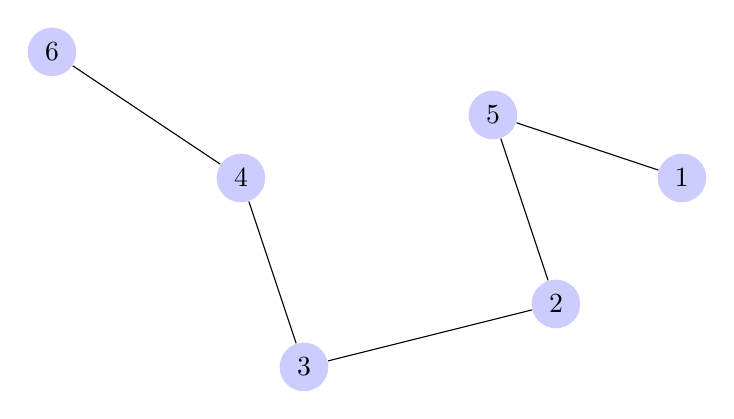
\begin{tikzpicture}
  [scale=.8,auto=left,every node/.style={circle,fill=blue!20}]
  \node (n6) at (1,10) {6};
  \node (n4) at (4,8)  {4};
  \node (n5) at (8,9)  {5};
  \node (n1) at (11,8) {1};
  \node (n2) at (9,6)  {2};
  \node (n3) at (5,5)  {3};

  \foreach \from/\to in {n6/n4,n5/n1,n2/n5,n2/n3,n3/n4}
    \draw (\from) -- (\to);

\end{tikzpicture}

%example diagram
%A labelled tree of size $n$ is a tree $T$ such that $|V(T)| = n$ and there exists a bijection between $V(T)$ and the set of natural numbers $\{1,2,3,\dots, n\}$. In particular we say that the node labelled 1 is the \emph{root} of the tree.  An increasing tree is a labelled tree such that the sequence of labels along any branch starting at the root is increasing. 

%Let $T$ be an increasing tree on $n$ nodes.  If distinct non-root nodes $u,v \in V(T)$ then we say that $u$ and $v$ live on the same \emph{branch} of $T$ if the sequence of vertices that comprise the unique shortest path between $u$ and $v$ does not include the root.
%make precise
%example
%The vertex set of the \emph{induced subgraph of a node} $m$ consists all vertices on the same branch of $m$ with higher or equal label than $m$.
%draw an example
%make precise

A \emph{random recursive tree} (RRT), $T$, with vertices $V(T) = \{v_{1},\dots,v_{n}\}$ is a 
labelled, rooted tree obtained by assigning a root vertex $v_{1}$ then adding $n-1$ vertices 
one by one such that each new vertex is joined by an edge to a randomly and uniformly chosen 
existing vertex. A random recursive $q$-ary tree is a labelled, rooted tree built in the same 
way as a random recursive tree except each new vertex is attached uniformly at random to an 
existing vertex that has outdegree less than $q$ \cite{Berg}.  We say that RRTs and random 
recursive $q$-ary trees are \emph{increasing} trees.  

Given an increasing tree $T_{n}$ on $n$ vertices labelled by the function 
$\phi : V(T) \rightarrow \{1,2,\dots,n\}$ and a vertex $v \in V(T)$ then we can consider 
$\tilde{T_{v}}$  which is the induced subtree with vertices, $v_{i}\in B(v)$ such that 
$\phi(v_{i}) \geq \phi(v)$. 

Given some tree $T$ we can formally measure how \emph{symmetric} that tree is by calculating 
the number of permutations of the vertices of that graph which preserves adjacent vertices.  
We call the set of all these permutations, $Aut(T)$, the \emph{automorphism group} of $T$ and 
the number of allowed permutations, $|Aut(T)|$ is the size of the automorphism group.  

\begin{ex}
Consider the following increasing tree $T_{14}$ with 14 vertices.  
\begin{figure}[H]
\centering
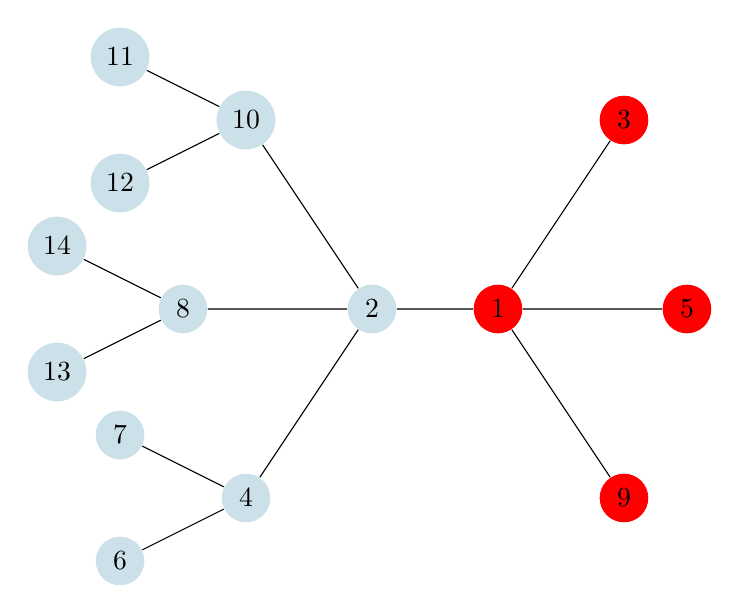
\begin{tikzpicture}
  [scale=0.8,auto=left,every node/.style={circle,fill=sotonblue!20}]

  \node[style={circle,fill=red!100}] (n1) at (7,5) {1};
  \node (n2) at (5,5)  {2};
  \node[style={circle,fill=red!100}] (n3) at (9,8)  {3};
  \node (n4) at (3,2) {4};
  \node[style={circle,fill=red!100}] (n5) at (10,5)  {5};
  \node (n6) at (1,1)  {6};
  \node (n7) at (1,3)  {7};
  \node (n8) at (2,5)  {8};
  \node[style={circle,fill=red!100}] (n9) at (9,2)  {9};considering
  \node (n10) at (3,8)  {10};
  \node (n11) at (1,9)  {11};
  \node (n12) at (1,7)  {12};
  \node (n13) at (0,4)  {13};
  \node (n14) at (0,6)  {14};
  \foreach \from/\to in {n1/n2,n1/n3,n1/n5,n1/n9,n2/n4,n2/n8,n2/n10,n10/n11,n10/n12,n8/n14,n8/n13,n4/n7,n4/n6}
    \draw (\from) -- (\to);
\end{tikzpicture}
\caption{}\label{fig2}
\end{figure}
The red vertices in Figure \ref{fig2} indicate an induced subtree $\tilde{T}_{v_{1}}$.  We can permute the 
vertices $v_{3},v_{5}$ and $v_{9}$, for example the following is a valid permutation of these 
vertices.
\begin{align*}
 3 \rightarrow 5\\
 5 \rightarrow 3\\
 9 \rightarrow 9 
\end{align*}
Note that after the above permutation all three vertices remain adjacent to $v_{1}$.  There are $3! = 6$
 distinct such permutations. The blue vertices in Figure \ref{fig2} highlight an extended 
symmetric induced subtree, 
$\tilde{T}_{v_{2}}$.  We can permute any of the pairs $\{v_{6},v_{7}\}, \{v_{11},v_{12}\}$ 
and $\{v_{13},v_{14}\}$ and we can permute the longer branches.  For example the following 
is a valid (adjacency preserving) permutation:
\begin{align*}
 4\rightarrow 8 \\
6 \rightarrow 13\\
7 \longrightarrow 14\\
8 \rightarrow 4\\
13 \rightarrow 7\\
14 \rightarrow 6
\end{align*}
Where every other vertex is fixed.  There are $X$ possible valid permutations of the blue 
vertices, therefore $|Aut(T_{14})| = 6 \times X = 6X$
\end{ex}

%ADD EXAMPLE
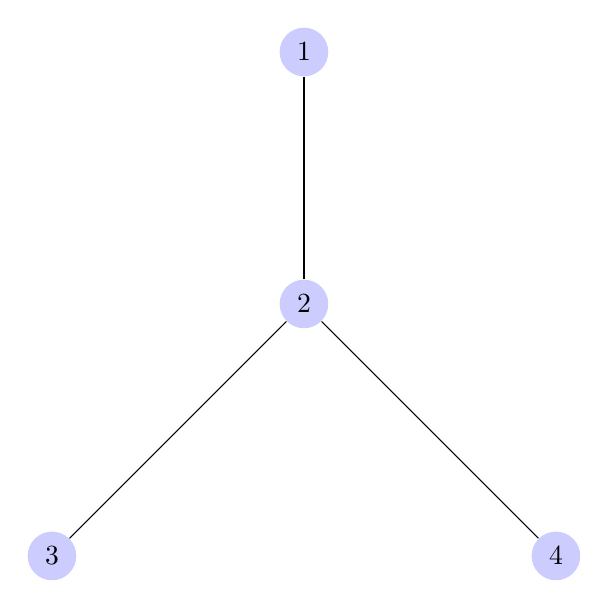
\begin{tikzpicture}
  [scale=.8,auto=left,every node/.style={circle,fill=blue!20}]
  \node (n1) at (6,10) {1};
  \node (n2) at (6,6)  {2};
  \node (n3) at (2,2)  {3};
  \node (n4) at (10,2) {4};
  

  \foreach \from/\to in {n1/n2,n2/n3,n2/n4}
    \draw (\from) -- (\to);

\end{tikzpicture}

\begin{figure}[H]

              \centering
%               \includegraphics[scale=0.3]{bifir.jpg}
                \caption{Perivascular drainage of A$\beta$.}
\end{figure}
\subsubsection{Anatomical Data}


 
In order to build an effective model we require anatomical data such as the expected length
 and radii of arterial vessels and the expected number of branching points.     

Note that 98\% of branching in the cerebral cortex is bifurcation and we expect approximately 
300 branching points \cite{Cassot}. 

Murray's principle of minimization of operational cost says that the cost of operation of
 physiological systems tends to a minimum.  One consequence of Murray’s principle is referred 
to as Murray's law which states that for $2$ daughter branches $d_{1}$ and $d_{2}$ from a 
common parent arterial vessel, $p$: 
\[r_{p}^{3} = r_{d_{1}}^{3} + r_{d_{2}}^{3}\]
where $r_{p}$ is the radius of $p$ and $r_{d_{1}},r_{d_{2}}$ are the radii of $d_{1}$ and 
$d_{2}$ \cite{Murray}.
Experimental evidence has shown that Murray's law is a good approximation for 
arterial vessels \cite{}.

Murray's law describes the relationship between particular vessels which can be thought of as 
\emph{cylinders}.  However, recall that our goal is to model the cerebral perivascular pathways
which can be thought of as \emph{annular prisms}.  Therefore we will adjust Murray's law to describe 
the relationship between parent and child annular prisms.  Since the notion of radius is more 
complicated for an annular prism it is appropriate to reformulate Murray's law in terms of 
cross-sectional area.   

We assume that the width of the perivascular space, $\epsilon$ is the same for any vessel from capillary to
 artery.  So let he parent vessel have radius $r_{p} = r_{p}' + \epsilon$ and the two 
daughter vessels have radii $r_{di} = r_{di}' + \epsilon$.
%insert diagram here
The relationship between the cross-sectional area, $A_{X}$ of any vessel and the radius, $r_{X}$ 
of that vessel is given by the formulae:
\begin{align}
 A_{X} &= \pi((r_{X}' + \epsilon)^{2} - r_{X}'^{2})\\
 &= \pi(\epsilon^{2} + 2\epsilon r_{X}')\\
 r_{X}' &= \frac{A_{X} - \pi\epsilon^{2}}{2\epsilon\pi}\\
 r_{X} &=  \frac{A_{X} - \pi\epsilon^{2}}{2\epsilon\pi} + \epsilon \\
 &= \frac{A_{X} + \pi\epsilon^{2}}{2\epsilon\pi}
\end{align}

By combining the above equations we find that the cross-sectional area of the parent
 vessel, $A_{p}$, is given by:

\begin{align}
A_{p} &= \pi(\epsilon^{2} + 2\epsilon r_{p})
&= \pi\left(\epsilon^{2} + 2\epsilon (r_{d_{1}}^{3} + r_{d_{2}}^{3})^{\frac{1}{3}}\right)
&= \pi\left(\epsilon^{2} + 2\epsilon \left(\left( \frac{A_{d_{1}} + \pi\epsilon^{2}}{2\epsilon\pi} \right)^{3} + \left( \frac{A_{d_{2}} + \pi\epsilon^{2}}{2\epsilon\pi} \right)^{3}\right)^{\frac{1}{3}}\right)
\end{align}
%\[A_{p} = \frac{((A_{1} - \epsilon^{2})^{3} +(A_{2} - \epsilon^{2})^{3})^{\frac{1}{3}}}{\epsilon} + \pi\epsilon^{2}\]
where $A_{d_{1}}$ and $A_{d_{2}}$ are the cross-sectional areas of the two daughter vessels.
%later we will chose epsilon to be one an initially set all leaves to have radius 300
\section{What we did}
We developed a program in Matlab \cite{} to model the role of symmetry in perivascular drainage. 
%do we need sample code here?
Firstly we built 50 random trees with 300 nodes and maximum valency 3.  These were obtained by beginning 
with a pair of nodes connected by an edge then at time $t$ a new edge connects node labelled $t$ to one of 
the existing %define existing
nodes with valency less than 3 uniformly at random.  

We then associated a capacity to each edge in the following way:
\begin{itemize}

\item[(i)] An edge with an endpoint that is a leaf is given capacity/volume 1 corresponding to radius $\frac{1}{\sqrt{\pi}}$.

\item[(ii)] We assume that all edges have length 1 and apply Murray's law for annuli to generate all other 
capacities.


\end{itemize}
For each tree $T$ we used nauty \cite{nauty} to calculate $aut(T)$.

We then activate our model by using the discrete variable $t$ where initially $t = 0$ and subsequently $t =
1,2,3,\dots$.

We define a variable, $v$, related to concentration. %Maybe read the literature to see what would be appropriate.
\[v = initial capacity/current capacity\]

As our model develops the capacity of the whole tree decreases because parts become "clogged up" so $v$ is 
monotonically increasing.

At each discrete time with probability proportional to $v$ we remove an edge and the induced subtree of 
$v$. This replicates CAA an amyloid plaque in a branch.  

We also record the time at which every edge has been removed from tree $T$ which we will refer to as the 
silting time.

Finally we split the trees into the 25 trees with largest automorphism group and 25 trees with smallest automorphism groups
and recorded the mean 

\section{Results}  
add my diagram.

We see that more symmetric trees take longer to fully silt (on average).  
\subsection{Interpretation of results}

Now we translate the mathematics back to biology.  Is it expected that more symmetric trees are more 
robust to this kind of attack?

Is there corroborating evidence from places who knows where!.

\section{Further Directions}
what about angiogenisis  - Ambrose


stiffening of arteries over time  - radial function decreases.
%simply percentages being decreased.
% consider this as a tree with $n$ edges where there was 1 edge last time  - then could play with the 
%cheegar constant as it would be important as the measure of bottle-necks - this is a good idea so d
%on't forget it!!!!!!!!!!!!!!!!!!!!!!!!!!!!!!!!!!!!!!!!!!!!!!!!!!!!
%what would the eigenspectrum tell us?  - bouds for cheeky cheegar. oh yer
Note that in the future lengths chosen from a probability spectrum would improve the matter.   


\bibliographystyle{h-physrev3.bst}
\bibliography{medicine}

\end{document}



A_{p} = \epsilon \pi \left( 2 \left(\left( \frac{A_{d_{1}} + \epsilon^{2}\pi}{2\epsilon\pi}\right)^{3} + \left( \frac{A_{d_{2}} + \epsilon^{2}\pi}{2\epsilon\pi}\right)^{3}\right)^\frac{1}{3} - \epsilon \right)
